


 
    \section{Cycles of science}
    \label{cycles}

        %How it all fits together.

Science connects us to the world. 
From \textit{scientia} to \textit{Wissenschaft}, science has ever connoted both sense and wisdom.
It is how humanity takes in from, and the arts are how humanity gives back to, nature.
Yet the neat duality of modern identity is no more mysterious than those in modern physics.
Experimental physics unites insight and craft: it makes tools of discovery.
As physicists, our aspiration to know the cosmos is realized if and only if that knowledge is both true and understood.

For the present, we do strive for gravitational wave astronomy to be understood, as in Chapter~\ref{chap7}.
Above all, we must know whether or not it is true.
The author's projects detailed in Chapters~\ref{chap2} through~\ref{chap6} explain how we may yet learn what is.

        \subsection{Improvements to observatories}
        \label{observatories_better}

           % Enhancements like enhanced/advanced LIGO and squeezing.
Gravitational wave interferometry is a young science.
The astrophysical potential is even more nascent.
First, we must have a view. 
Chapter~\ref{chap2} details how the LIGO Scientific Collaboration is reaching out to our colleagues in the astronomical community to unite our view of the universe.
The author also discusses contributions made to characterizing the LIGO Hanford Observatory, building a phase camera for use in future interferometers, and studying detector glitches.
Chapter~\ref{chap4} shows that more fundamental improvements are possible.
By way of quantum optical squeezing, the standard quantum limits of the electromagnetic field can be surpassed.
Using squeezing \textit{in lieu} of laser power, the observatory reached unprecedented sensitivity.

        \subsection{Understanding instruments, refining data}
        \label{instrumental_understanding_data_refinements}

            %....necessitate detector characterization, like scans and filters
            %....automated feedforward filters yield own enhancements

        %\subsection{Refining data}
        %\label{data_refinements}

Detector characterization has its own enhancements to give to LIGO.
Chapter~\ref{chap3} explains how the couplings between the auxiliary length controls and the gravitational wave strain introduce unwanted noise -- and how it can be subtracted.
Great care is taken to ensure that these fixes do not add any noise or unphysical signal.
These methods can both be applied \textit{post facto} and, without the surrounding machinery, in real-time.
The author's work began at the end of the last science run, S6, and similar techniques may make such challenges a smaller obstacle in the future.
Advanced observatories are becoming complicated instruments: we need means to see and disentangle the ties between their parts.

        \subsection{Searching deep-space}
        \label{searching_space}

        %    ...TwoSpect and other searches benefit
Even the quietest, most sensitive gravitational wave interferometer is uninteresting if we cannot understand it.
There are four key ways to listen to the gravitational wave sky: inspirals, bursts, stochastic, and continuous wave.
Our search in Chapters~\ref{chap5} and~\ref{chap6} has been for the last: continuous waves from neutron stars in binary systems.
TwoSpect is already a capable search for unknown systems across the entire sky; the author modified the search to focus on Scorpius X-1 and XTE J1751-305, having honed methods on a simulated set of data in collaboration and competition with fellow searchers.
These preliminary results will soon be presented and appear to be best so far for frequencies above 500 Hz.

        \subsection{Reaching out, looking up}
        \label{reaching_out}

         %   ...Outreach makes research accessible to public.
The sky excites the mind.
Just as astronomy with light and X-rays, radio waves and neutrinos has caught the popular imagination, it is the hope of projects like those in Chapter~\ref{chap7} to inspire others to ponder gravitational wave astronomy.
While increasingly confident in the sources we see, the adventure lies in the unknown.
The author has shown a simple and effective tool, a model interferometer, for showing a new kind of antenna, a new sort of observatory, to search out that unknown.

    \section{Scientific merit: filtering and analysis}
    \label{merit}

        %Core projects.

        \subsection{Feedforward improvement to LIGO data}
        \label{feedforward_end}

         %   Evaluate success of feedforward.
Quantitative enhancements to LIGO are hard.
The LIGO Scientific Collaboration is composed of over a thousand scientists, and most contributions are indirect.
Feedforward subtraction of auxiliary channel noise is a rare case where an individual can directly improve the scientific power of a gravitational wave interferometer operating at full sensitivity.
This algorithm enhanced inspiral range by about four percent in S6, potentially allowing twelve percent more inspiral events to be detected.

More exciting still is the community forming behind a family of related techniques.
Automated subtraction of a large class of noise sources -- not only length control but glitches, gravitational gradients, and Schumann resonances of the Earth's magnetic field -- could be cancelled, according to work underway by fellow LIGO researchers.
One of the author's chief interests in this project was in proving that such a technique can be both effective and safe for the data.
We believe that this has been shown.

        \subsection{TwoSpect directed search for neutron stars in binary systems}
        \label{TwoSpect_end}

          %  ...and TwoSpect-directed.

           % One thought that might develop into something more fruitful is as follows.

            %Someday deconvolve, maybe Bayesian, the skymaps and parameter space spread of TwoSpect with simulation to understand what we are really seeing. Cannot do all templates in paramter space, but only need a few to compare -- in a way, it already does.

Detecting gravitational waves is not easy, or else it would have been done long ago.
Nonetheless, our algorithms, like our observatories, are better than they have ever been.
The TwoSpect search has evolved into a form suitable for searching Scorpius X-1 and XTE J175301-305, and for the latter is close to establishing a 95\% confidence upper limit on random polarization gravitational waves as low as $1.3\times10^{-24}$. 
%Contigent on reconciliation with other searches, this may prove the best limit so far.

TwoSpect is already prepared for better data to arrive when Advanced LIGO begins observing runs in 2015.
Indeed, enhancements are possible between now and then that may make it yet more capable.
Neutron stars, the heaviest compact objects entirely in our universe -- black holes in some sense having left the universe behind -- remain opaque to our scrutiny for now.
Gravitational waves will unveil some of their secrets.
%The pull of neutron stars gathers many disciplines together that they shine more brightly, and perhaps a jet will be shot off to launch physics in new directions. 

    \section{Entering the advanced detector era}
    \label{advanced_detector_era}

        %Advanced LIGO: how much better can we do?

Second-generation interferometers, Advanced LIGO and its peers, are almost here. 
Both LIGO Hanford and LIGO Livingston have completed installing all their components, have sealed their vacuum, and are actively commissioning.
Advanced Virgo is also underway.
Tunnels for KAGRA have been completed.
Gravitational waves may not yet be seen for several years, and perhaps only faintly at first.
As a fellow scientist\footnote{Brian O'Reilly of Livingston.} noted, Kepler saw two supernovae in the Milky Way in his lifetime; there have been none since.
Perhaps we will be profoundly unlucky.
Yet we have planned with circumspection and care for what we think we can expect: if two neutron stars merge within 200 Megaparsecs of Earth, then our observatories, by decade's end, should hear that inspiral.
The bursts of supernovae and bumps on neutron stars will be sensible too, and, in time, the Big Bang.
Even if we fail to see these (it would require much inspection and introspection before we are certain there is nothing to be seen), something will be learnt.
Should more be there than we expect, then all our curiosity will be justified.

    \section{Vision of a dark sky}
    \label{dark_sky}

\begin{figure}
\begin{center}
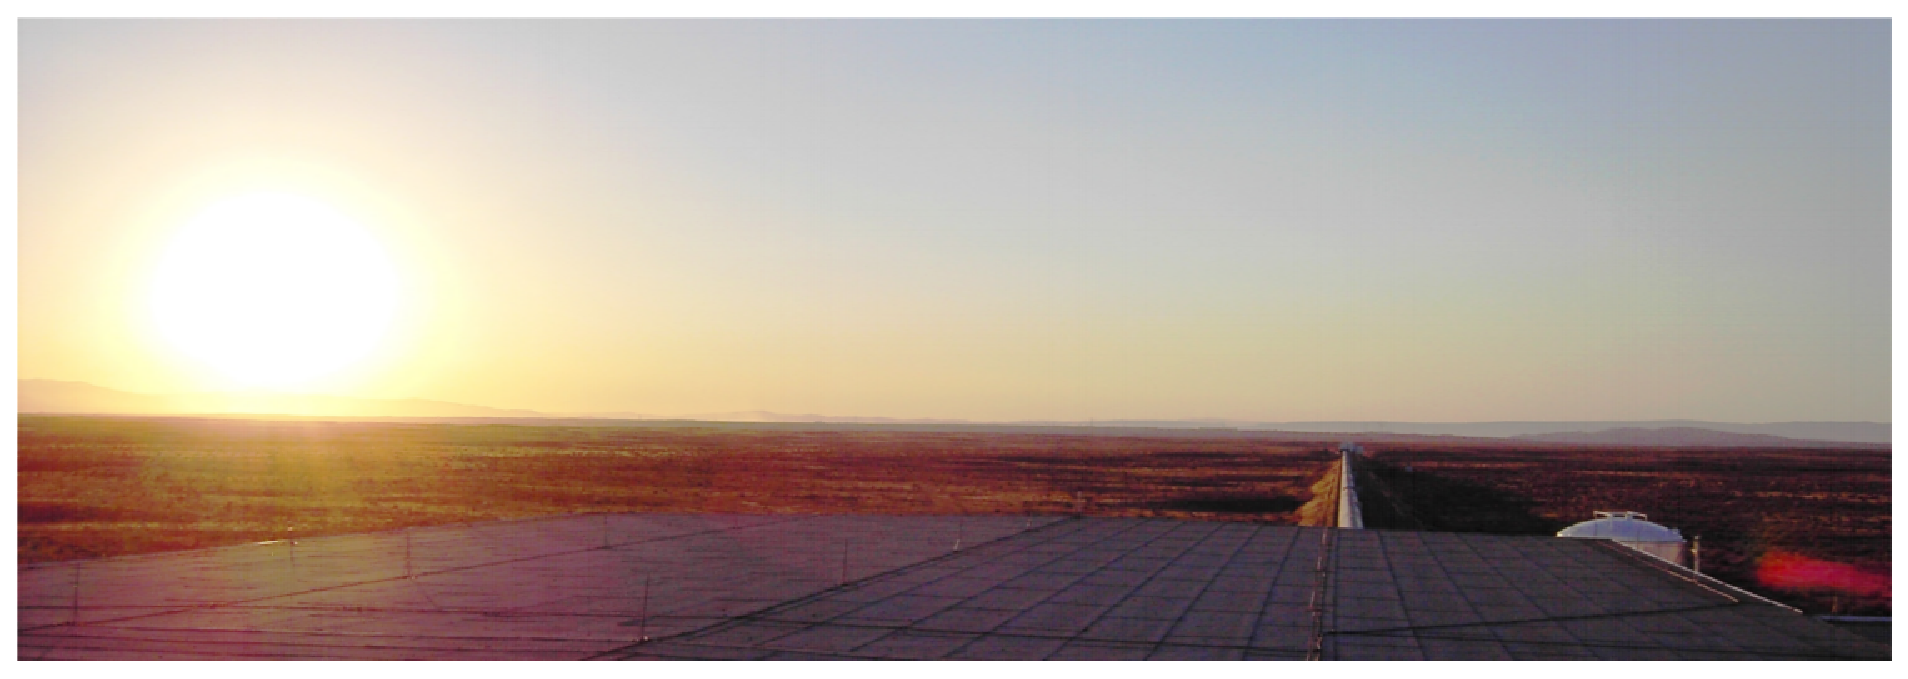
\includegraphics[height=50mm,width=148mm]{LIGOpanoramasmall.eps}
\caption{LIGO Hanford Observatory sunset, inital detector era. Photo by author. Like the Hanford desert wiped clean by the Missoula floods, the gravitational wave sky may relate cosmic tales of cataclysm and rebirth in the distant past.}
\label{LIGO_panorama_small}
\end{center}
\end{figure}

        Why gravitational wave astronomy at all? What could be out there?

        Gravity is the universe. At the dawn of the twenty-first century, the Standard Model of physics, and quantum field theory in general, can be studied on curved spacetime, but the spacetime itself remains scarcely better understood than when Einstein first proposed it general relativity. 
After almost a century, the fabric of the universe is still unyielding of its secrets. 
Gravitational wave astronomy will be the first science to perceive that fabric directly. 

        In this thesis, we have made inroads to this new astronomy. Superficially seperate, the common thread is the pursuit of fundamental issues by skillful choice of perspective. 
With squeezing, the optical experimenter views a gravitational wave interferometer as a quantum system and sees how fluctuations in the vacuum, not just in the laser, create noise -- which can be cancelled with a beam of no-light.
With feedforward, the noise due to intrinsic couplings between the interferometer servos is found by coherence in the frequency domain -- and cancelled with subtraction that can take place either in real-time or long afterward.
With TwoSpect, signals buried beneath noise are uncovered by comparing multiple instruments -- cancelling noise, in effect, with the build-up of signal in other observatories.
Communicating these advances to a wider world is the final question of fundamental issues and choice of perspective.
Gravitational wave observations have not yet seen a signal, yet we find ways to make our research meaningful.

Until we can understand gravity, we will be ignorant to the range of forces present in the cosmos.
LIGO is a way to hear the echoes of gravitation.
For long-lasting signals, we can even `see' them, just as our ears can echolocate sounds.
 From the windswept, tumbleweed-coated plains of Hanford and the pine forests of Livingston may emerge our first visions of this thus-far dark sky. 
From it may come unexpected sources. 
Even if, though, we see only what we imagine will be seen, the insight into the hearts of neutron stars, the explosions of giant suns, the collisions of black holes, and the earliest, as-yet opaque instants of the primordial universe will be wonder enough. 
The author hopes to have contributed in some small way to this project. 

  
% Document Control Center, DCC, information:
% Directed searches for continuous gravitational waves from spinning neutron stars in binary systems 
% LIGO DCC-P1400102

%        -------------------------------------
%
%	The following is an example of using the commands \textit{ref}
%	and \textit{label}. With these commands theorems, chapters,
%	sections and figurres can be labeld with names in the tex file
%	and then refered to by these names in later tex files. In
%	chapter~\ref{intro} we saw section~\ref{sample_section} or
%	theorem~\ref{sample_theorem}.
%
%	Lastly, here is how to include a figure. First generate an
%	encapsulated postscript file in xfig, adobe illustrator or
%	some other program. The specific commands are found in
%	\textit{chap2.tex}.
%
%        \begin{figure}[htb]
%        \centerline{ \epsfig{figure=sample.eps, 
%        height =  1.5 in}}
%        \caption{Sample Figure}
%        \label{sample_figure}
%        \end{figure}

